\section{\Large KINEMATICS}
\subsection{Quaternions}
We choose a nominal attitude parameterization of quaternions, our choice being based on the absence of singularities. The following function computes the time derivative for a state consisting of quaternions (4 parameters) and angular velocity (3 parameters).

The equations below describe the propagation of kinematics using quaternions.
\begin{align*}
\Vec{\Omega} &= 
    \begin{bmatrix}
    0 & \omega_{z} & -\omega_{y} & \omega_{x}\\
    -\omega_{z} & 0 & \omega_{x} & \omega_{y}\\
    \omega_{y} & -\omega_{x} & 0 & \omega_{z}\\
    -\omega_{x} & -\omega_{y} & -\omega_{z} & 0
    \end{bmatrix}\\
\frac{d \Vec{q}}{dt} &= \frac{1}{2} \Vec{\Omega} \Vec{q}(t)
\end{align*}
The following script shows the computation of the time derivative for quaternions

\lstinputlisting{src/kinQuaternion.m}

We can use the previous function to perform a forward Euler numerical integration. We call the previous function over a fixed time step to compute the evolution of the state.

\lstinputlisting{src/kinQuaternionForwardEuler.m}

For improved precision, we implement a 4th order Runge-Kutta method, which uses a weighted sum of slopes to obtain a better result. This also calls the time derivative function, but does so with different values of the state, which are weighted to obtain the next state for each step.

\subsection{Euler Angles}
Similarly, we create a function that computes the time derivative of a state consisting of Euler angles and angular velocity using the 3-1-3 symmetric Euler angle sequence.

The equations for the propagation of kinematics for Euler angles are below.
\begin{align*}
\frac{d \phi}{dt} &= \frac{\omega_{x} \sin(\psi) + \omega_{y} \cos(\psi)}{\sin(\theta)}\\
\frac{d \theta}{dt} &= \omega_{x} \cos(\psi) - \omega_{y} \sin(\psi)\\
\frac{d \psi}{dt} &= \omega_{z} - (\omega_{x} \sin(\psi) + \omega_{y} \cos(\psi)) cot(\theta)
\end{align*}
\lstinputlisting{src/kinEulerAngle.m}

We can propagate this with forward Euler, as in the previous section.

\lstinputlisting{src/kinEulerAngleForwardEuler.m}

For our actual implementation, we choose to use the time derivative function with \texttt{ode113} for improved accuracy. Note that this cannot be done as simply for quaternions, as they require normalization at each step, hence our decision to implement RK4.

\subsection{Integration of Attitude Parameterizations}
We integrate our attitude parameterizations (including angular velocity using Euler equations).

\begin{figure}[H]
\centering
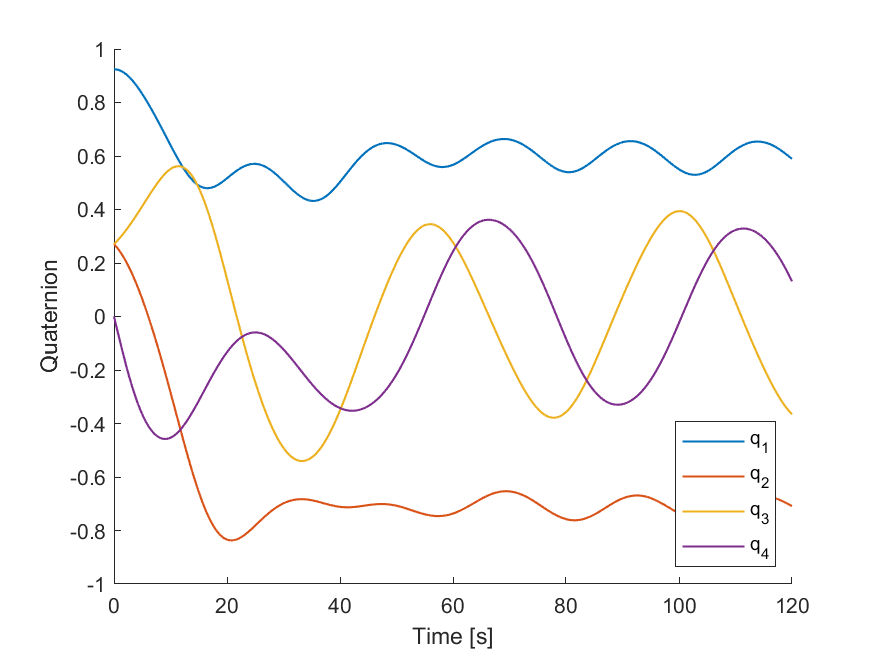
\includegraphics[scale=0.6]{Images/ps3_problem6_quaternions.png}
\caption{Evolution of quaternions}
\label{fig:ps3_problem6_quaternions}
\end{figure}

\begin{figure}[H]
\centering
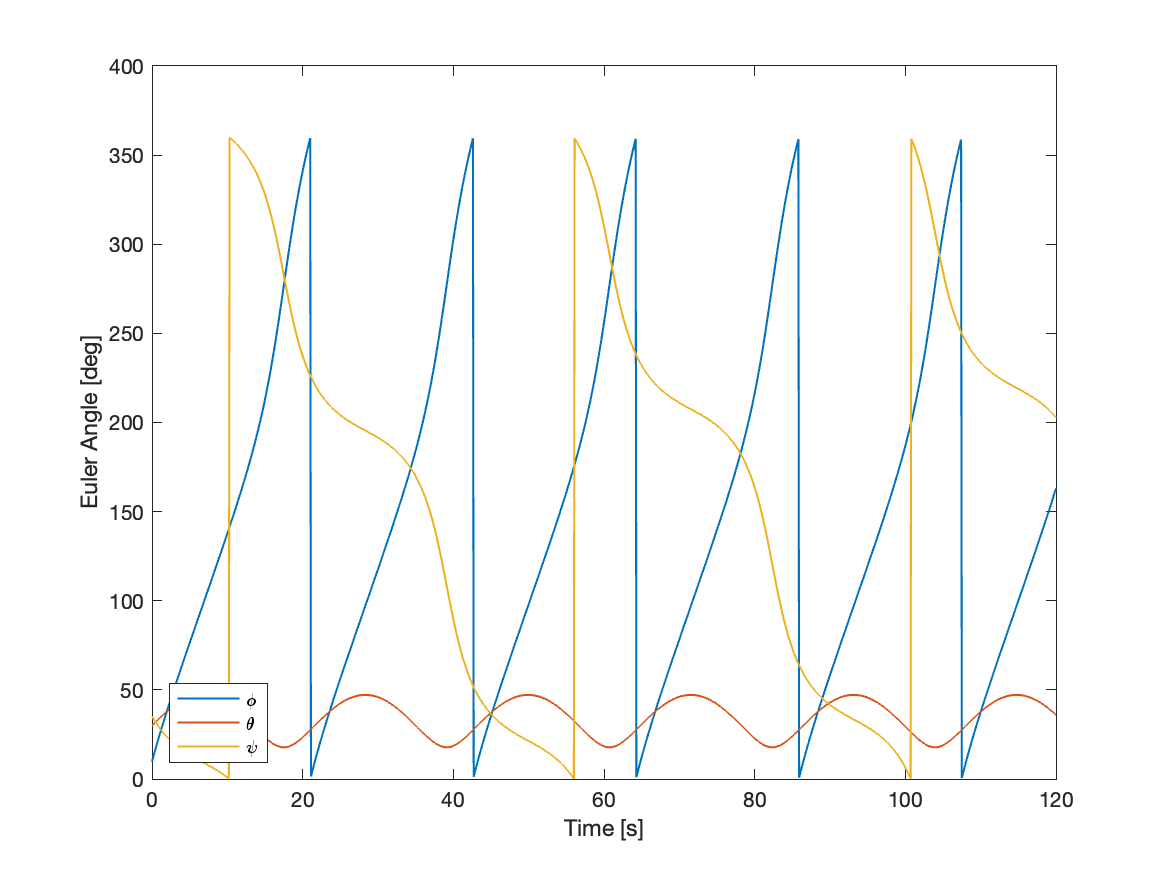
\includegraphics[scale=0.6]{Images/ps3_problem6_euler.png}
\caption{Evolution of Euler angles}
\label{fig:ps3_problem6_euler}
\end{figure}

\subsection{Angular Momentum Vector}
Figure \ref{fig:ps3_problem7a} shows the components of the angular momentum vector over time, as computed from our primary attitude representation of quaternions. The angular momentum vector (and its individual components) remains constant in the absence of external torques.

\begin{figure}[H]
\centering
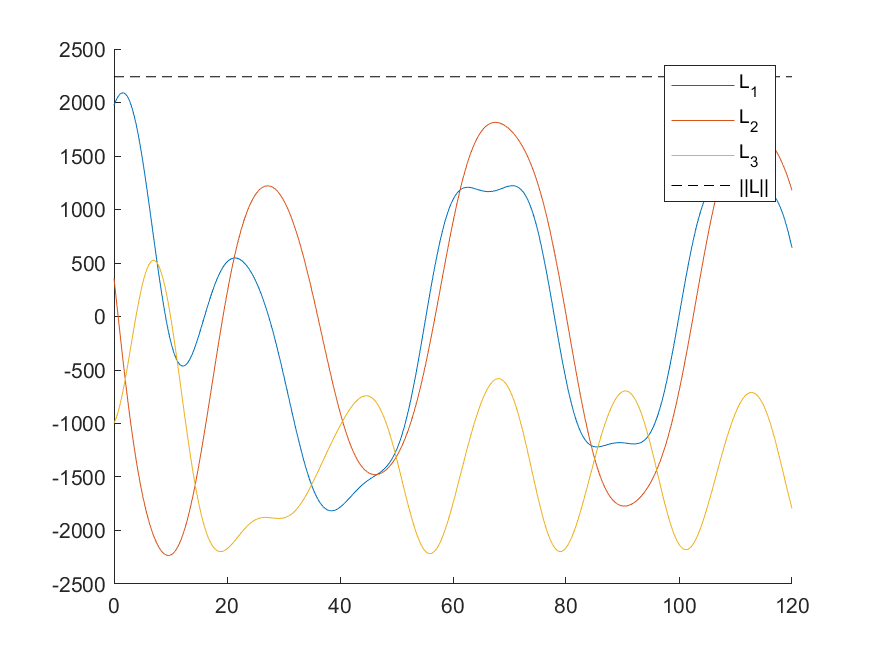
\includegraphics[scale=0.6]{Images/ps3_problem7a.png}
\caption{Angular momentum in inertial coordinates is constant}
\label{fig:ps3_problem7a}
\end{figure}

Figure \ref{fig:ps3_problem7b} shows the angular momentum and angular velocity vectors overlaid with the herpolhode. The animation (see caption) shows the evolution of the herpolhode and provides a better visualization of the herpolhode's geometry. 

\begin{figure}[H]
\centering
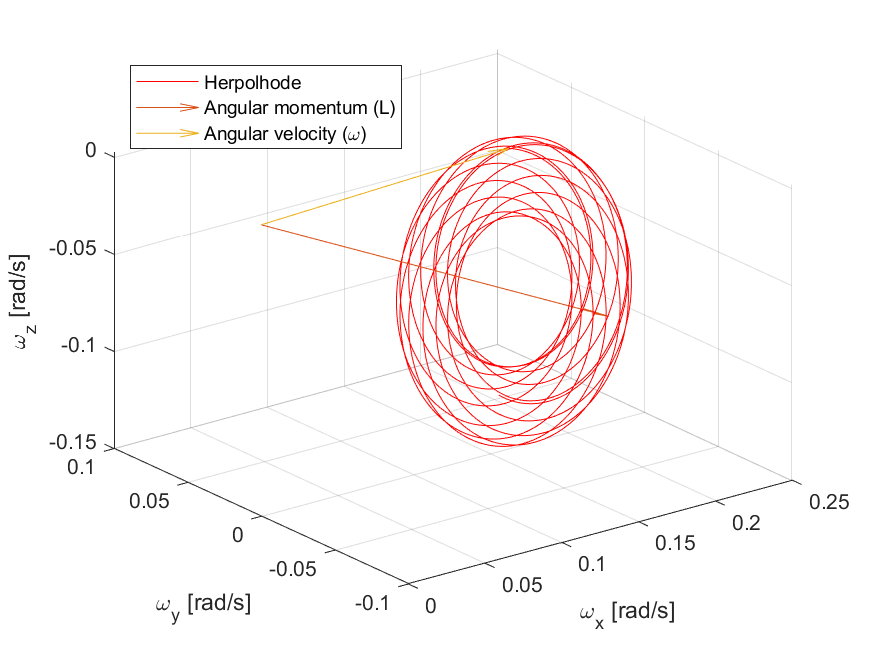
\includegraphics[scale=0.6]{Images/ps3_problem7b.png}
\caption{Herpolhode (Animated: \protect\url{https://tinyurl.com/herpolhode})}
\label{fig:ps3_problem7b}
\end{figure}

Figures \ref{fig:ps3_problem7c_rtn}, \ref{fig:ps3_problem7c_body}, and \ref{fig:ps3_problem7c_principal} include the plots of the orbital (RTN), body, and principal axes over the course of a single orbit. The RTN frame varies with rotation about the orbit, while rotation can be seen in the body and principal axis plots based on the rotation in our initial condition.

\begin{figure}[H]
\centering
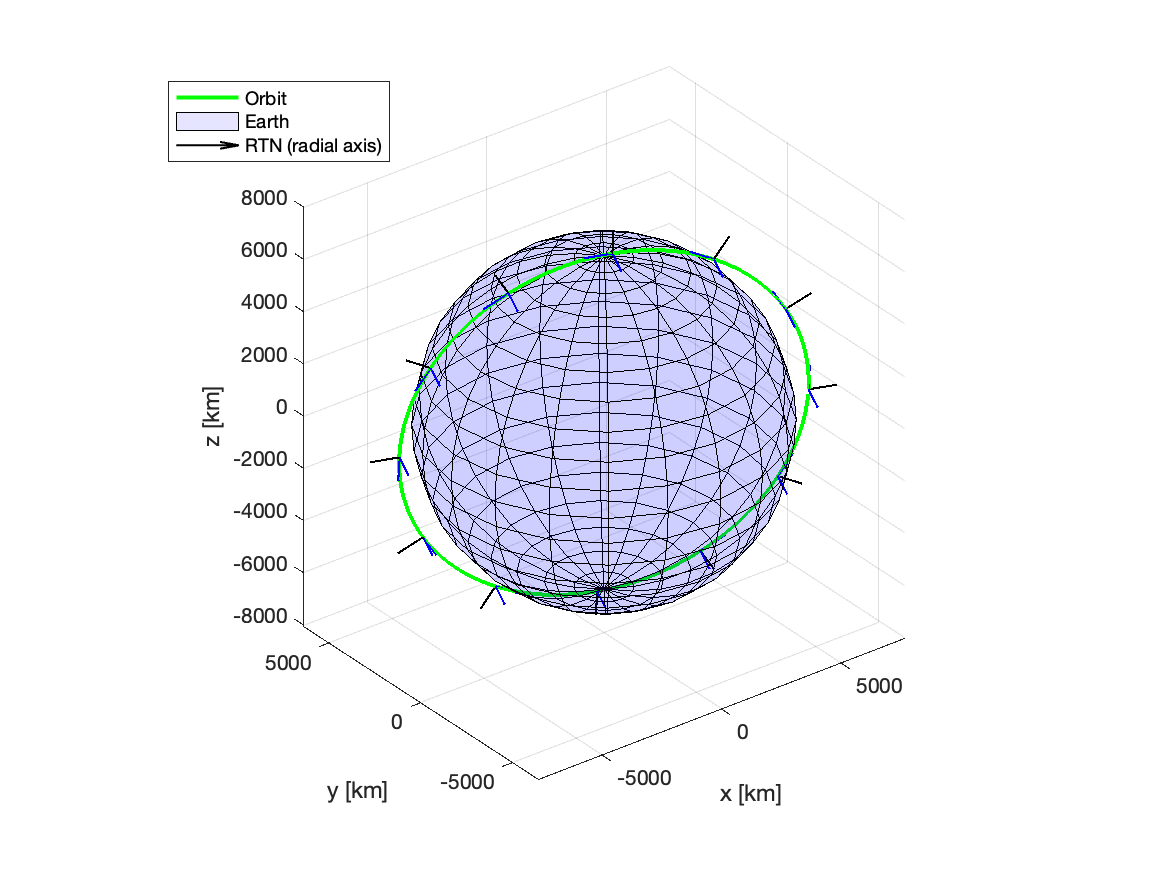
\includegraphics[scale=0.7]{Images/ps3_problem7c_rtn.png}
\caption{Propagation of RTN frame}
\label{fig:ps3_problem7c_rtn}
\end{figure}

\begin{figure}[H]
\centering
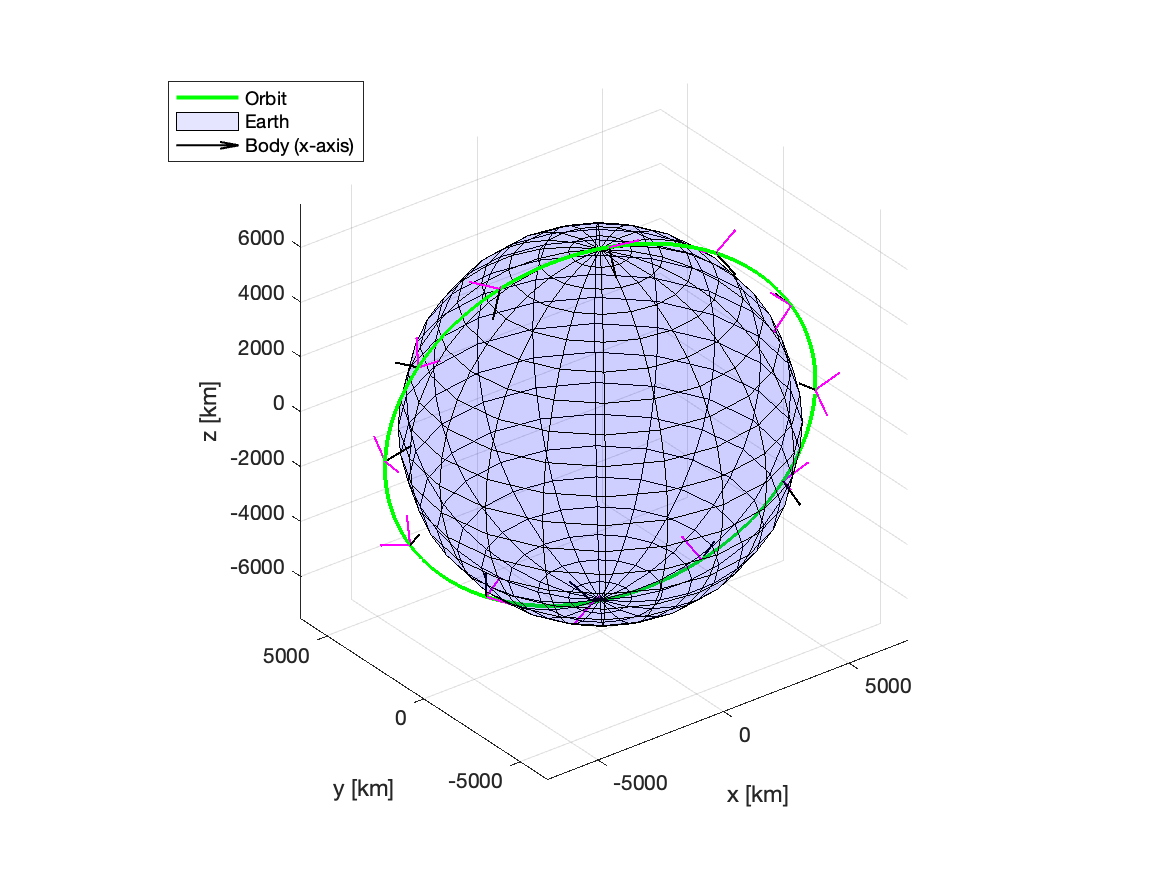
\includegraphics[scale=0.7]{Images/ps3_problem7c_body.png}
\caption{Propagation of body axes}
\label{fig:ps3_problem7c_body}
\end{figure}

\begin{figure}[H]
\centering
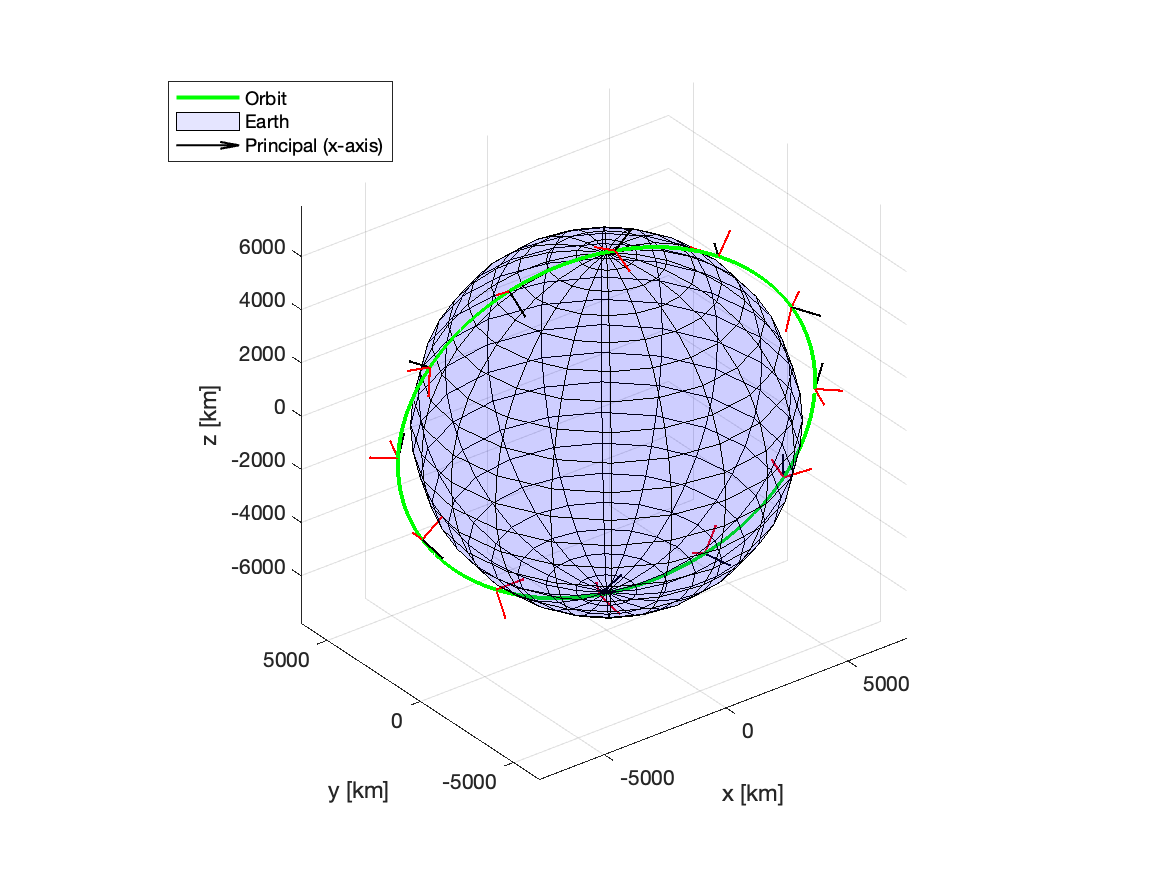
\includegraphics[scale=0.7]{Images/ps3_problem7c_principal.png}
\caption{Propagation of principal axes}
\label{fig:ps3_problem7c_principal}
\end{figure}

\subsection{Stability, Inertial}
We assume that two components of the initial angular velocity are zero and that the principal axes are aligned with the inertial frame. This is an equilibrium state. To test the equilibrium state, we choose the following initial angular velocity,
\begin{align*}
\Vec{\omega} &= 
\qty[parse-numbers = false]{
    \begin{bmatrix}
    0 \\
    0 \\
    1 \\ 
    \end{bmatrix}
}{\radian\per\s},
\end{align*}
and we set all Euler angles to zero. We use a 312 convention for Euler angles, which avoids singularities for this configuration.

Figure \ref{fig:ps4_problem1a_angvel} shows results of the simulation, where $\omega_x$ and $\omega_y$ remain zero and $\omega_z$ maintains a constant value.

\begin{figure}[H]
\centering
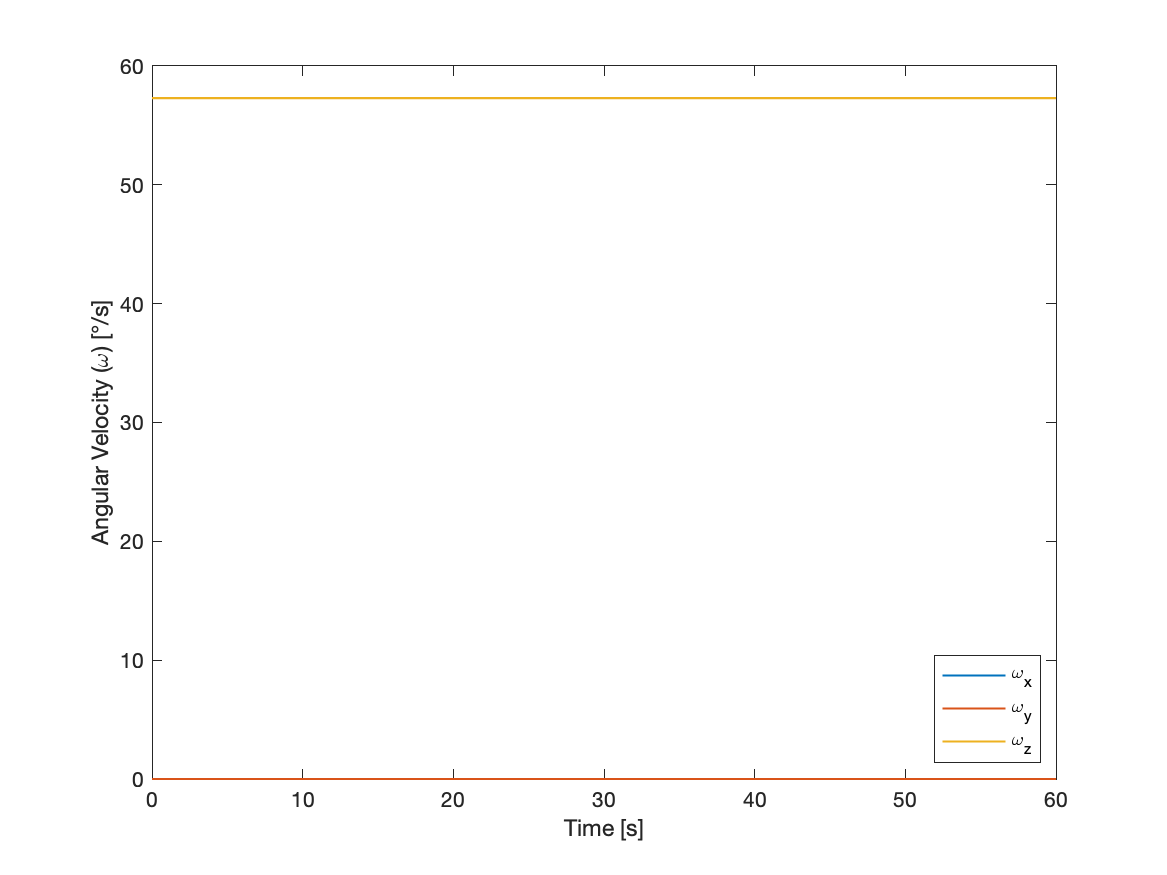
\includegraphics[scale=0.6]{Images/ps4_problem1a_angvel.png}
\caption{Evolution of angular velocity}
\label{fig:ps4_problem1a_angvel}
\end{figure}

Similarly, in Figure \ref{fig:ps4_problem1a_angle}, $\phi$ and $\theta$ Euler angles remain at zero while the $\psi$ Euler angle increases linearly.

\begin{figure}[H]
\centering
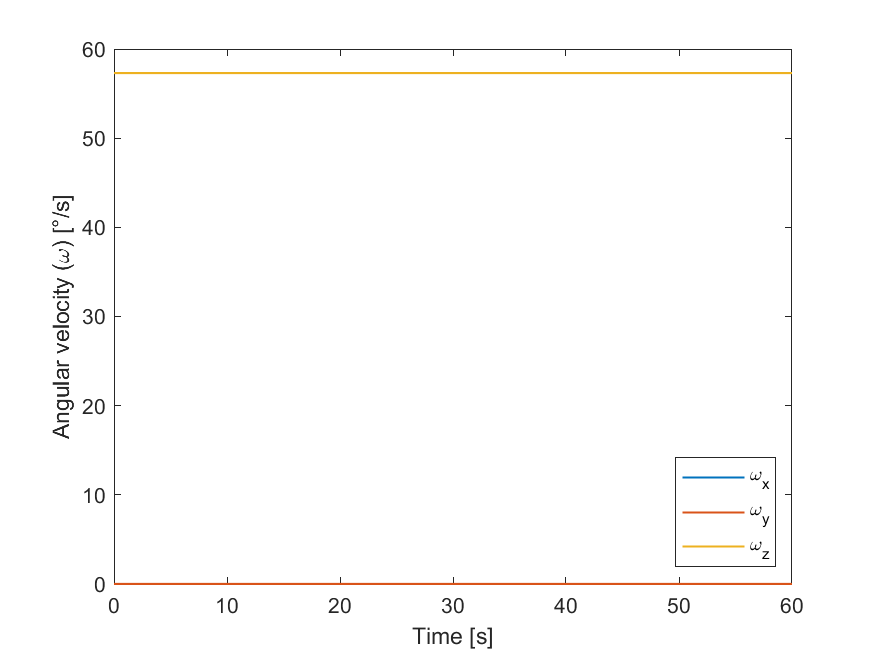
\includegraphics[scale=0.6]{Images/ps4_problem1a_angle.png}
\caption{Evolution of Euler angles}
\label{fig:ps4_problem1a_angle}
\end{figure}

\subsection{Stability, RTN}
Now, we choose to align our principal axes with the RTN frame. For selected initial orbital conditions taken from the NISAR science users' handbook, we obtain the initial position and compute the RTN frame, which we then use to find initial aligned Euler angles.

\begin{figure}[H]
\centering
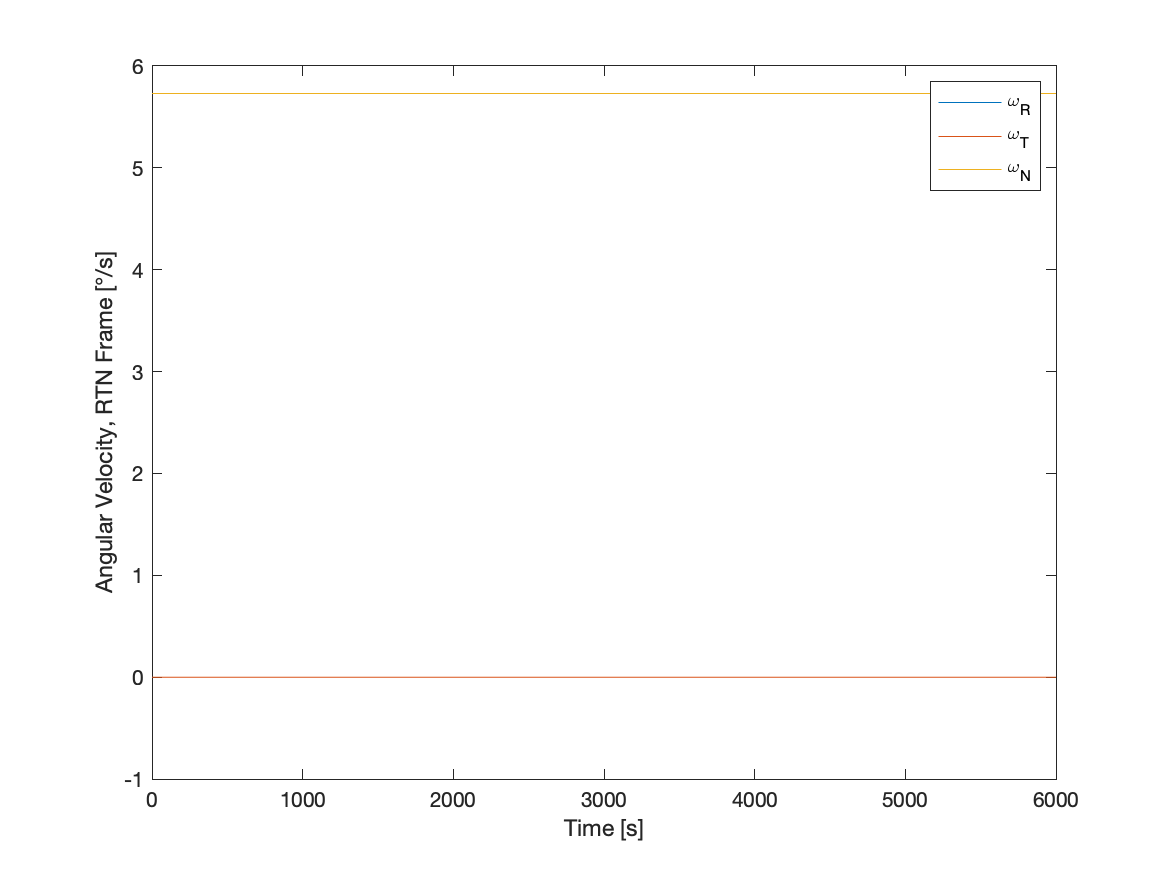
\includegraphics[scale=0.6]{Images/ps4_problem1b_angvel.png}
\caption{Evolution of angular velocity}
\label{fig:ps4_problem1b_angvel}
\end{figure}

We set a nonzero $\omega_z$ angular velocity, which is aligned with the normal direction of the RTN frame, and we choose all other angular velocities to be zero. Propagating the orbit and attitude, we find that the angular velocity remains constant throughout the orbit, even relative to the RTN frame, as seen in Figure \ref{fig:ps4_problem1b_angvel}. From Figure \ref{fig:ps4_problem1b_euler}, we see that the $\theta$ and $\psi$ Euler angles related to the RTN frame are constant while $\phi$ varies.

\begin{figure}[H]
\centering
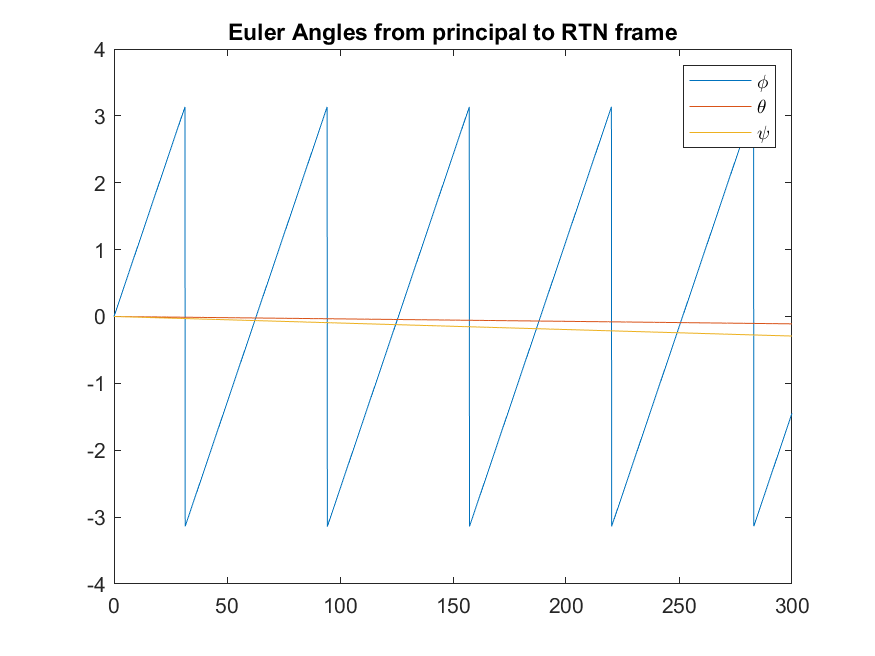
\includegraphics[scale=0.6]{Images/ps4_problem1b_euler.png}
\caption{Evolution of Euler angles}
\label{fig:ps4_problem1b_euler}
\end{figure}

This result shows our satellite's maximum inertia principal axis remains aligned with the normal direction of the orbit such that the maximum inertia principal axis remains normal to the plane of the orbit, given the initial condition that axes are aligned with the RTN frame and angular velocity along other axes is nonzero.

\subsection{Stability, Single-Spin}
For a single spin satellite, the three possible equilibrium configurations are rotation about the minimum inertia principal axis, rotation about the intermediate axis, and rotation about the maximum inertia principal axis. Figures \ref{fig:ps4_problem2a_1}, \ref{fig:ps4_problem2a_2}, \ref{fig:ps4_problem2a_3} show that the Euler angles are stable about the minimum and maximum axes, but it is unstable about the intermediate axes. This is as expected for our system, with the minimum and maximum axes exhibiting periodic stability with small oscillations in angular velocity.

\begin{figure}[H]
\centering
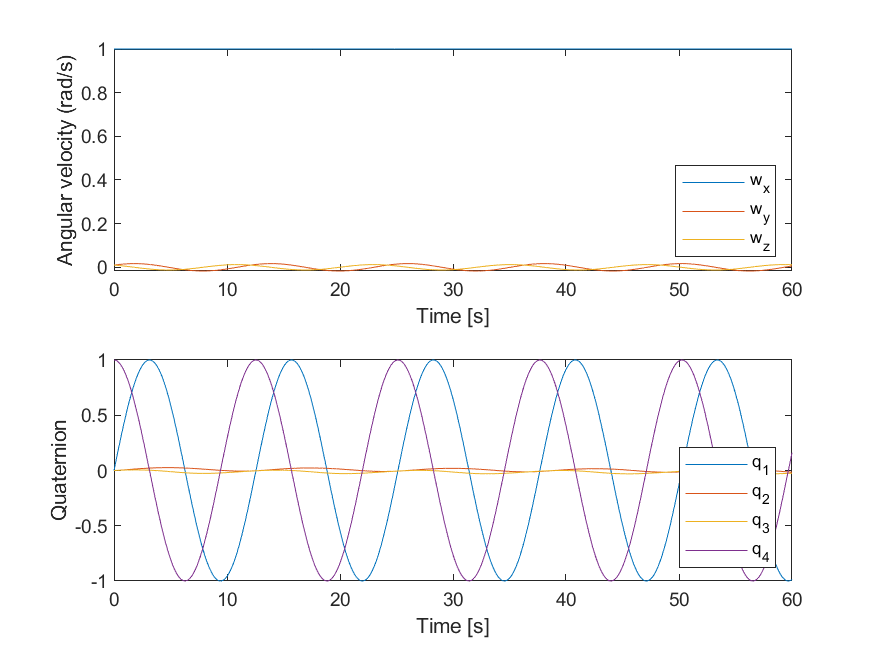
\includegraphics[scale=0.6]{Images/ps4_problem2a_1.png}
\caption{Simulation of satellite spinning on its minimum principal axis}
\label{fig:ps4_problem2a_1}
\end{figure}

Note that while in Figure \ref{fig:ps4_problem2a_1} the angular velocities are periodically stable, the Euler angles oscillate. This is likely a consequence of the sequence of rotations used for our choice of Euler angle convention.

\begin{figure}[H]
\centering
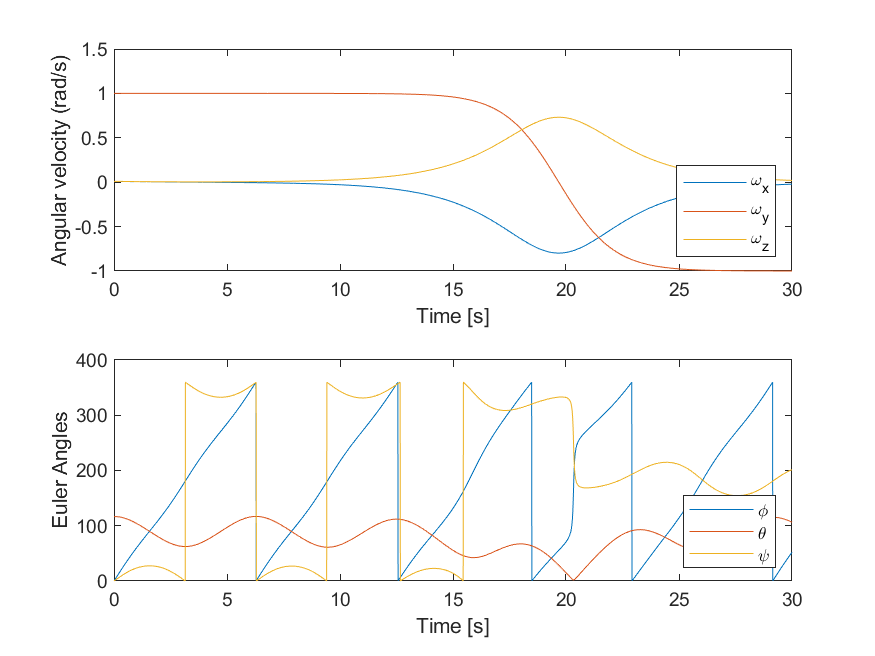
\includegraphics[scale=0.6]{Images/ps4_problem2a_2.png}
\caption{Simulation of satellite spinning on its intermediate principal axis}
\label{fig:ps4_problem2a_2}
\end{figure}

\begin{figure}[H]
\centering
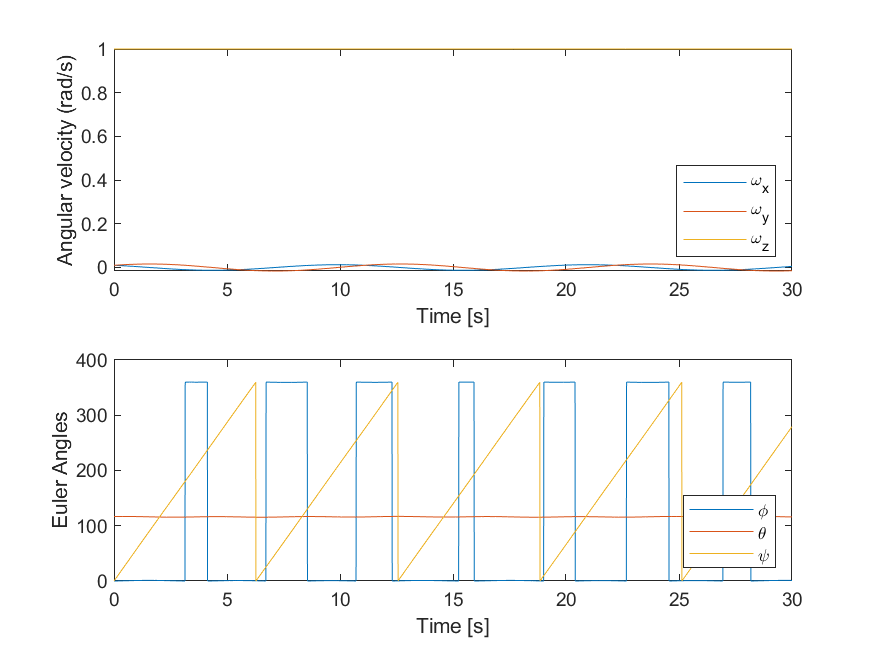
\includegraphics[scale=0.6]{Images/ps4_problem2a_3.png}
\caption{Simulation of satellite spinning on its maximum principal axis}
\label{fig:ps4_problem2a_3}
\end{figure}

\subsection{Stability, Dual-Spin}
We select a momentum wheel similar to our mission specifications to model a dual-spin satellite.

We choose to use specifications from the RSI 68 momentum wheel, for which datasheets are readily available online \cite{RSI68}. This particular momentum wheel is intended for spacecraft in the 1,500 to 5,000 kg range, which matches our mission. We use a diameter of 347 mm and mass of 8.9 kg and model our reaction wheel as a hoop with mass concentrated about the outer diameter. We also use 2,500 RPM, which yields approximately the nominal angular momentum from the datasheet–the maximum angular velocity is 6,000 RPM. The following Euler equations are used to model a momentum wheel as a rotor. For this problem, we set the torques on the right side of each equation to zero, as we are not considering external torques.
\begin{align*}
    I_x \dot{\omega_x} + I_r \dot{\omega_r} r_x + (I_z - I_y) \omega_y \omega_z 
    + I_r \omega_r (\omega_y r_z - \omega_z r_y) = M_x \\
    I_y \dot{\omega_y} + I_r \dot{\omega_r} r_y + (I_x - I_z) \omega_z \omega_x 
    + I_r \omega_r (\omega_z r_x - \omega_x r_z) = M_y \\
    I_z \dot{\omega_z} + I_r \dot{\omega_r} r_z + (I_y - I_x) \omega_x \omega_y 
    + I_r \omega_r (\omega_x r_y - \omega_y r_x) = M_z \\
    I_r \dot{\omega_r} = M_r
\end{align*}
The function \texttt{kinEulerAngleWheel}, shown below, is used in addition to \texttt{ode113} to simulate the angular velocities over time.

\lstinputlisting{src/kinEulerAngleWheel.m}

Simulating the Euler and kinematic equations, Figure \ref{fig:ps4_problem3b} shows the angular momentum vector remain constant in the inertial frame, as expected.

\begin{figure}[H]
\centering
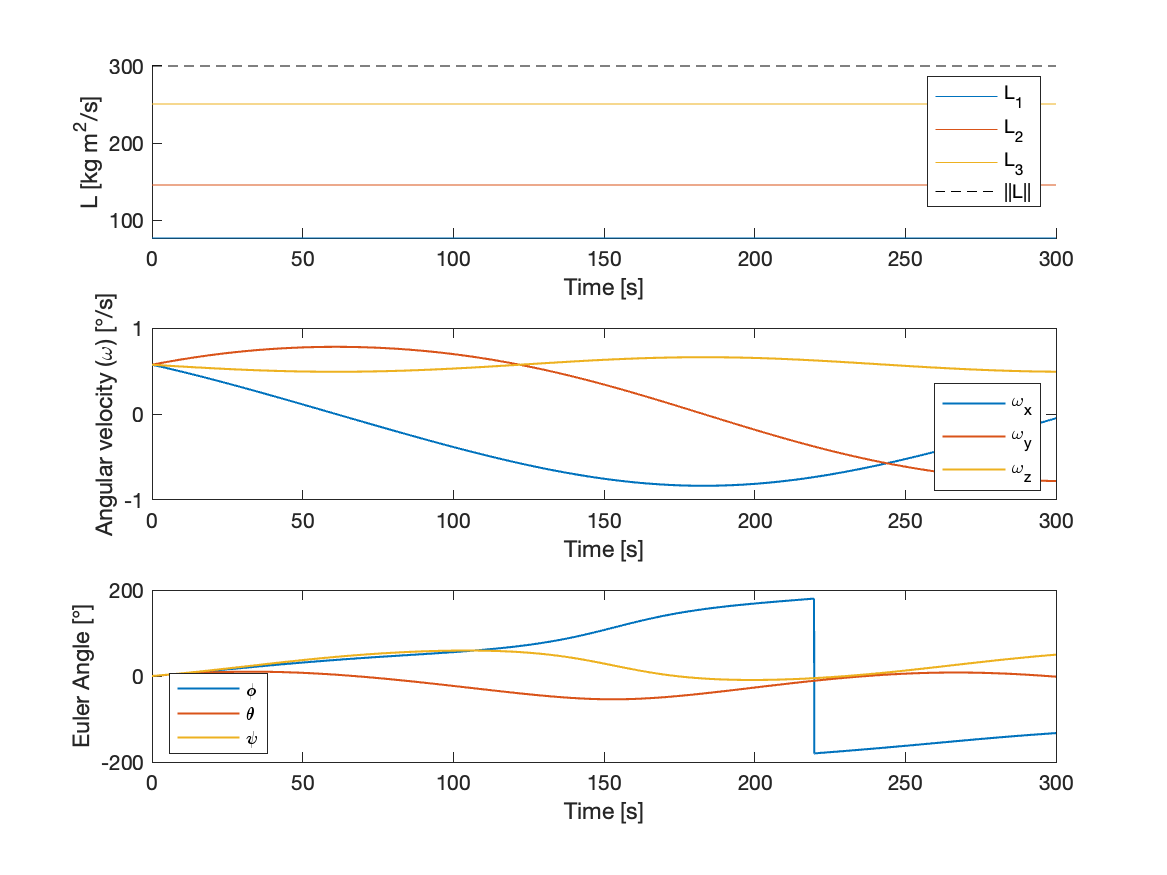
\includegraphics[scale=0.6]{Images/ps4_problem3b.png}
\caption{Angular momentum conserved with angular momentum components constant}
\label{fig:ps4_problem3b}
\end{figure}

By linearizing the Euler equations about equilibrium, the following result shows that periodic stability (in this case, about the z-axis) can be met with a reaction wheel if one of the following conditions are met:
\begin{align*}
    1)\; I_r \omega_r > (I_y - I_z) \omega_z \;\; AND \;\; I_r \omega_r > (I_x - I_z) \omega_z \\
    2)\; I_r \omega_r < (I_y - I_z) \omega_z \;\; AND \;\; I_r \omega_r < (I_x - I_z) \omega_z
\end{align*}
We demonstrate equilibrium and stability for this new system with the reaction wheel. Figures \ref{fig:ps4_problem3c_x.png}, \ref{fig:ps4_problem3c_y.png}, \ref{fig:ps4_problem3c_z.png} show the analysis for each of the principal axes. As before, the minimum and maximum inertia principal axes are periodically stable, but the intermediate axis is unstable.

This behavior resembles that found previously. In this case, we perturb each angular velocity as well as the rotor angular velocity. Our rotor velocity in this case is not enough to stabilize spin about the intermediate axis.

\begin{figure}[H]
\centering
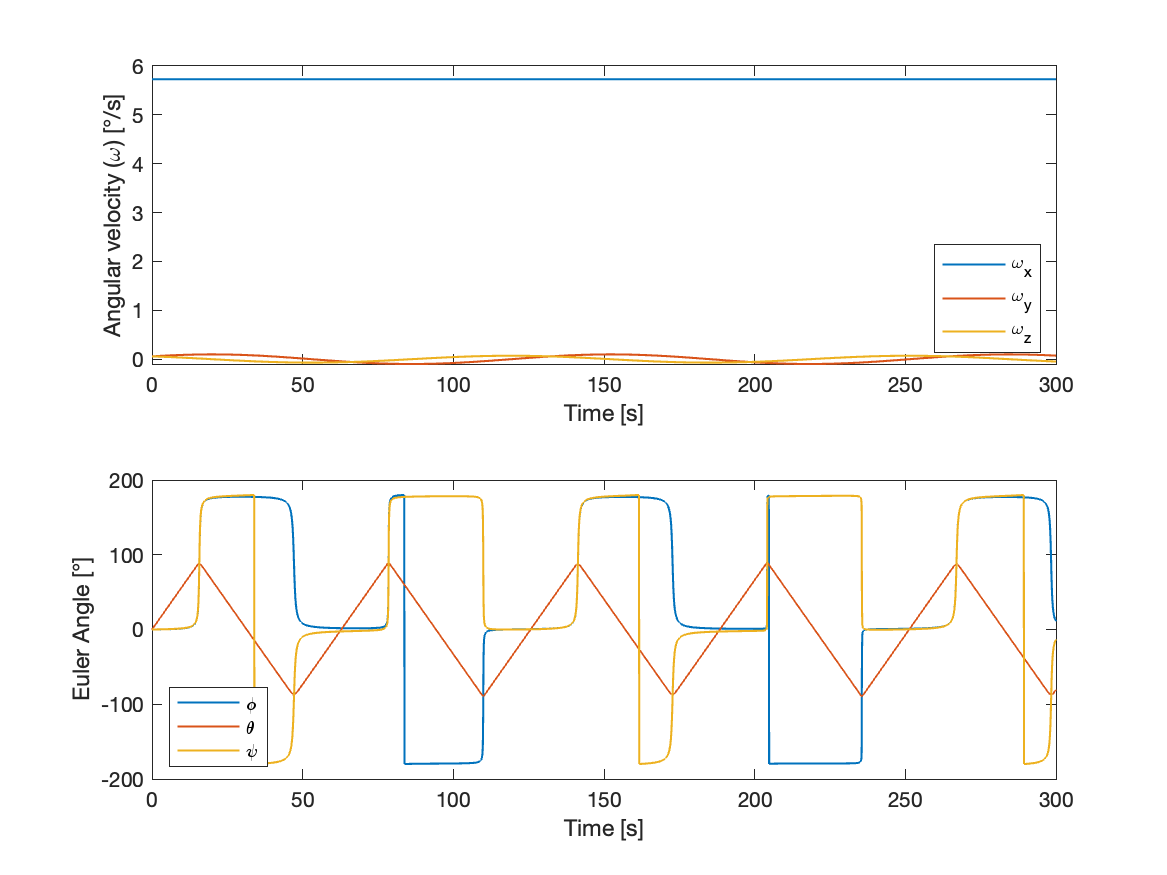
\includegraphics[scale=0.6]{Images/ps4_problem3c_x.png}
\caption{Stability analysis about minimum inertia principal axis}
\label{fig:ps4_problem3c_x.png}
\end{figure}

\begin{figure}[H]
\centering
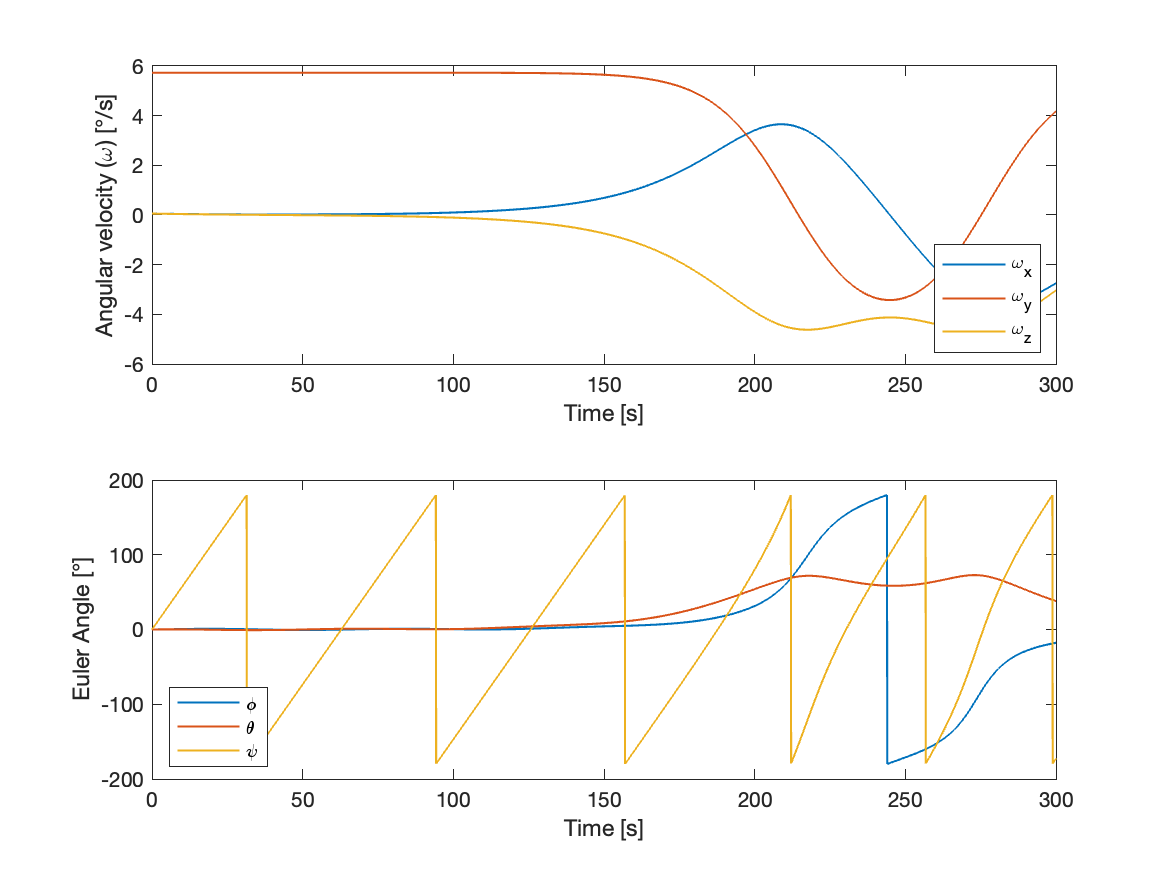
\includegraphics[scale=0.6]{Images/ps4_problem3c_y.png}
\caption{Stability analysis about intermediate axis}
\label{fig:ps4_problem3c_y.png}
\end{figure}

\begin{figure}[H]
\centering
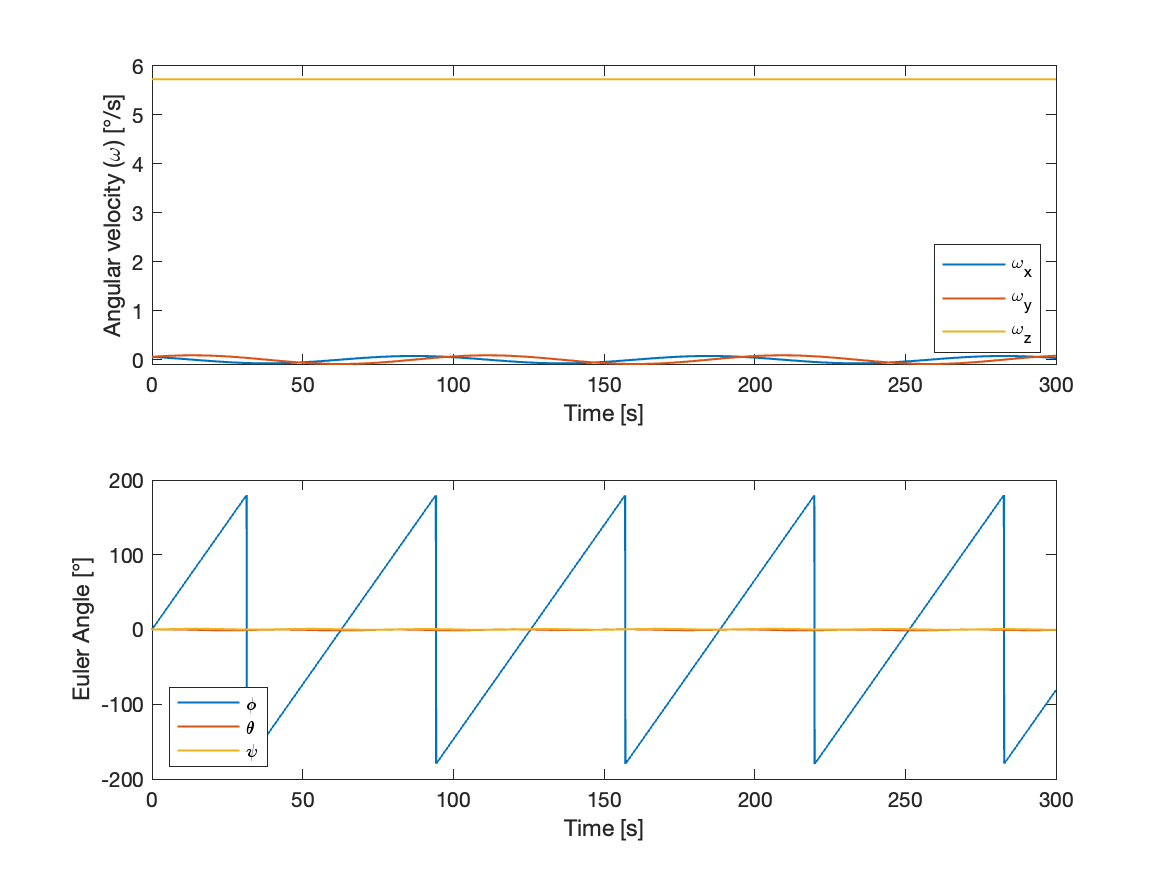
\includegraphics[scale=0.6]{Images/ps4_problem3c_z.png}
\caption{Stability analysis about maximum inertia principal axis}
\label{fig:ps4_problem3c_z.png}
\end{figure}

Using the stability condition, we can make the attitude motion stable. In our case, increasing the angular velocity of the rotor by a factor of 10 obtains a stable system for spin about the intermediate axes.

\begin{figure}[H]
\centering
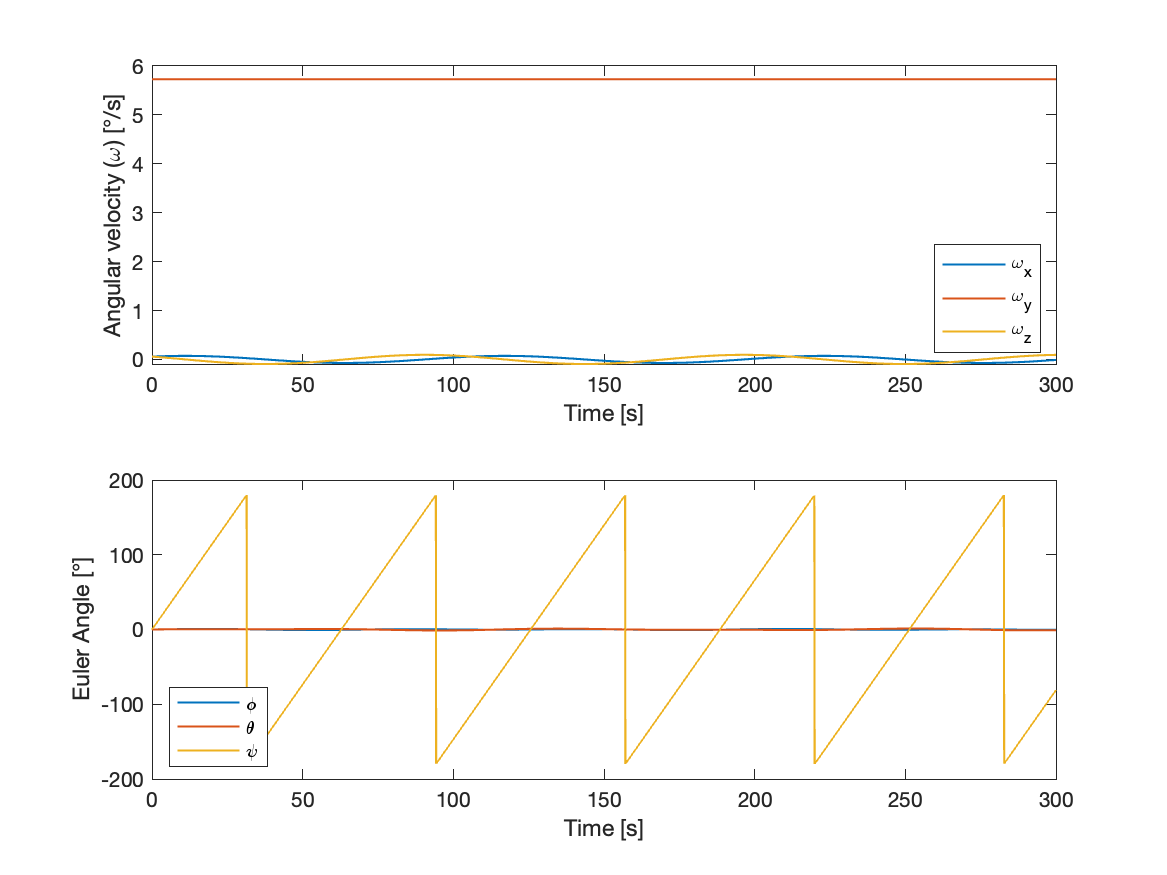
\includegraphics[scale=0.6]{Images/ps4_problem3d.png}
\caption{}
\label{fig:ps4_problem3d.png}
\end{figure}

For the purpose of our mission, we choose to stabilize spin about the body x-axis, which is important for pointing our satellite and appropriately sweeping the target with our SAR. We use the rotation previously found between the principal and body axes to achieve this, applying the rotation to the angular velocity and the angular momentum vector direction of the momentum wheel.

\begin{figure}[H]
\centering
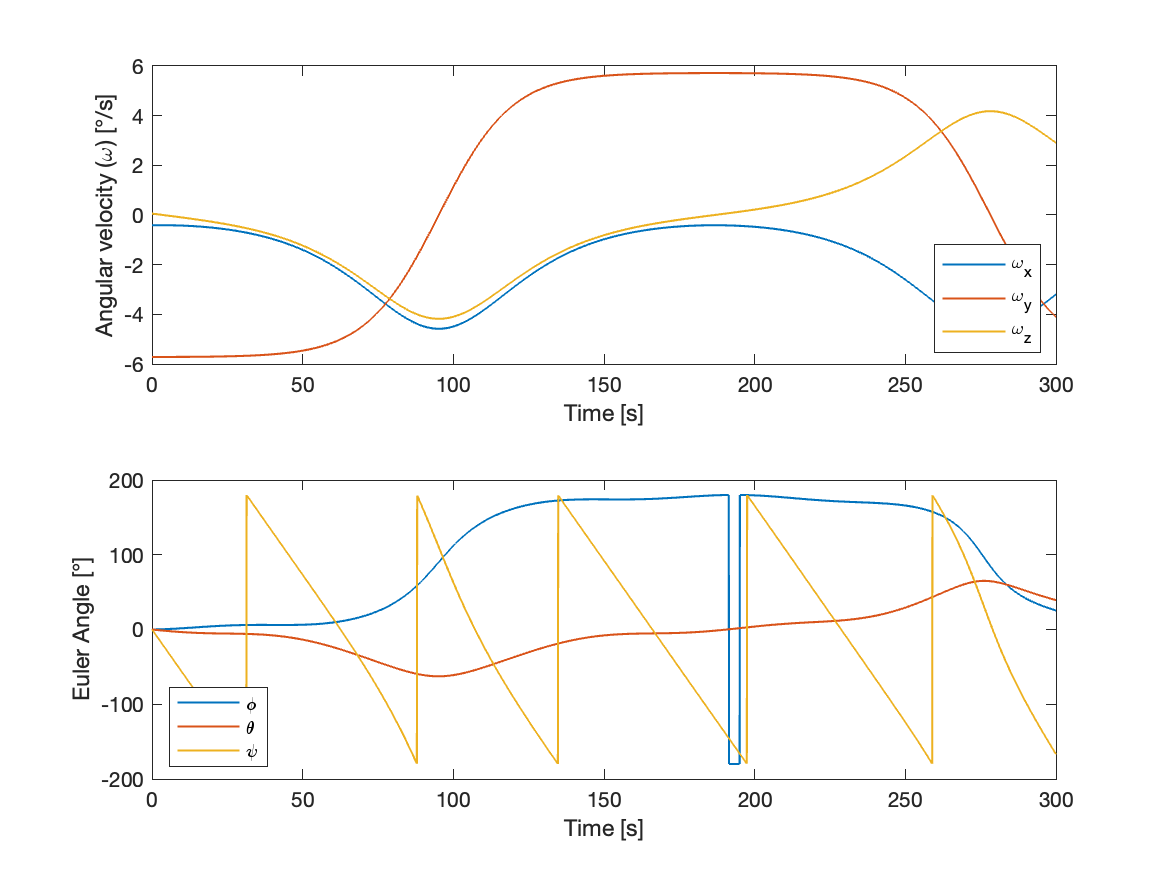
\includegraphics[scale=0.6]{Images/ps4_problem3e_unstable.png}
\caption{Initially unstable attitude with low momentum wheel angular velocity}
\label{fig:ps4_problem3e_unstable.png}
\end{figure}

\begin{figure}[H]
\centering
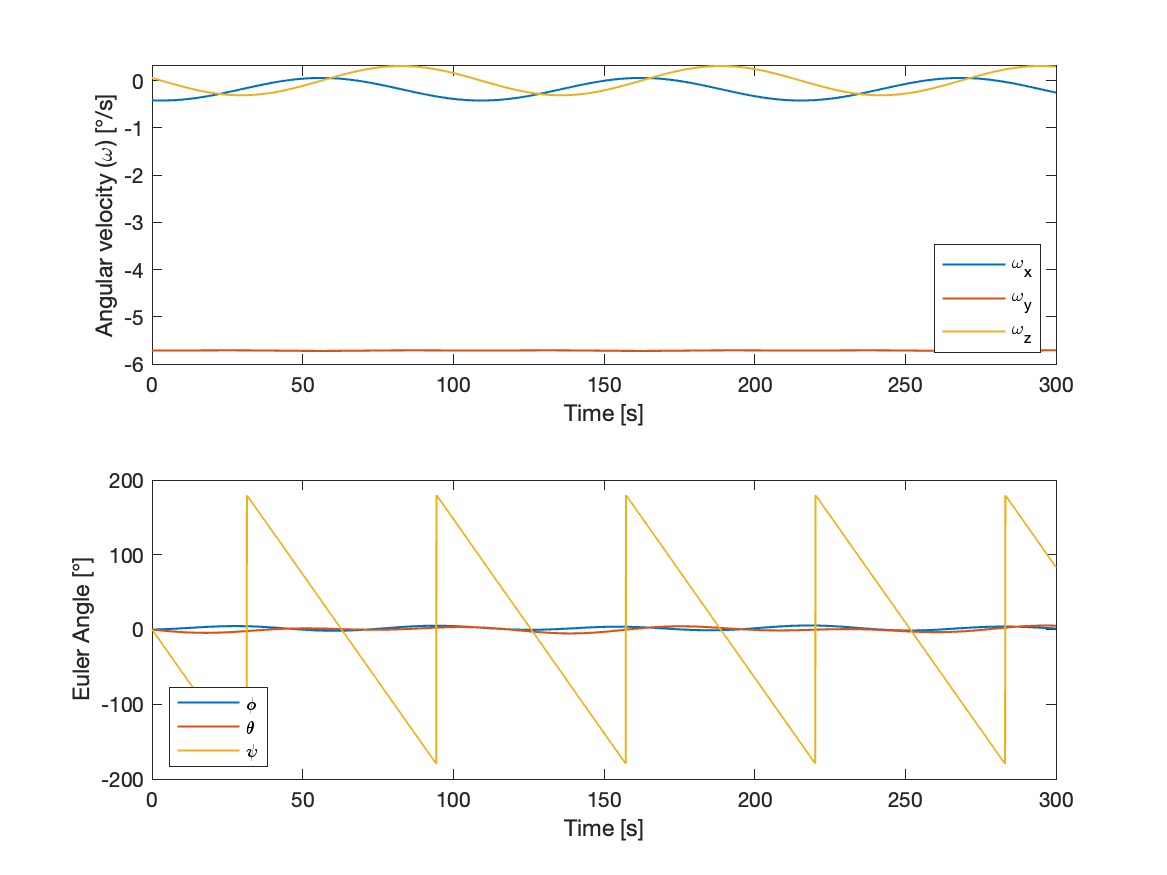
\includegraphics[scale=0.6]{Images/ps4_problem3e_stable.png}
\caption{Periodically stable attitude after increasing momentum wheel angular velocity 10x}
\label{fig:ps4_problem3e_stable.png}
\end{figure}